\chapter{Defining the system}

The definition of the system plays a crucial role as it essentially sets the
scene for the whole study. With the general goal of investigating the frictional
behvaiour of a graphene sheet as we alter it through kirigami cuts and stretch,
two different approaches was considered as sketched in
\cref{fig:system_variations}. One apprach is simply to mimic a \acrshort{FFM}
type experiment as done in most other numerical studies of friction. In this
case, we can probe the graphene sheet, resting on a substrate, with some sort of
indenting tip connected to a moving body representing a cantilever setup.
Friction is then measured by making the tip scan across the graphene surface.
This setup alows for for a variety tip shapes and sizes, and alternatively it
could bed broadened a flat surface making the setup resemble a \acrshort{SFA}
experiment. However, this approach seemmingly call for a fixed amount of
streching of the graphene sheet as it is pre-stretch before being attatched to
the substrate. Another option is therefore to attatch the graphene sheet to the moving body instead. The key different is then, that introduce some sort of nanomachine in the moving body which convert a normal load into a stretching motion. This gives more design room to utilize any stretch-related friciton effects that require a dynamical changing of the stretch amout as opposed to only being applied to keep the sheet and a certain stretch amount throughout the loading.


% Thus, if any interesting effects from stretch is found this can be utilized through such a nanomachine and be coupled to the loading which makes for a more complete metamaterial design. 

% . Now the contact surface is exclusively between the graphene sheet and the substrate, and we can stretch the sheet to different lengths before running the simulation. However, the key difference lies in the prospect for how we can utilize any interesting behvaiour related to the stretching of the sheet. By imagening that the moving body has a nanomachine feature that translates normal force to stretching we can design a system where the sheet is stretched upon loading. This leaves room for  a
% nanomachine setup where the sheet is changeing with load and a more interesting potential for applying any found effects. This is the main argument for choosing the latter approach, even though that this sets the system further apart from previous studies of friction in general.

% Note also that this changes from the substrate to the moving body carrying the interesting part .

% We can flip the system and attatched it to the substrate as well..

\begin{figure}[H]
  \centering
  \includegraphics[width=0.8\linewidth]{figures/system/system_variations.png}
  \caption{\hl{TMP} System variations}
  \label{fig:system_variations}
\end{figure}

Hence, using the second option our system of choice consist of two seperate parts: A 2D graphene sheet and a 3D Silicon ``bulk'' substrate. Note, that we do attempt to model the nanomachine explicitly in this study, but we will consider the prospects of adding this in \cref{chap:negative_fric}. 

% By applying a normal force and a tangential force we can investigate the friction behvaiour of the contact interface between the sheet and substrate.

% which interact through \acrshort{LJ} potential modelling a van der Waals force. 

\section{Region definitions}
Despite having two distinct parts of the simmulation, the sheet and the substrate, we provide a further subdivision ino specific regions according their functionality in the \acrshort{MD} simmulations. We denote the start end end regions of the sheet, with respect to one direction, as so-called \textit{pull blocks}, which is reserved for the application of normal load, stretching and
dragging of the sheet and applying the thermostat. The remaining \textit{inner
sheet} is left for the kirigami cuts and simulated as an $NVE$ ensemble. The pull blocks are equal split between a thermostat part and a rigid part. The rigid part is part of the thermostat during an initial relaxtion period before it is then made rigid for the final duration of the simulation. Note that the rigid parts on both sides of the sheet is then considered as a single rigid object even though
they are physically seperated. This means that all force interactions on these
parts will be applied as a common average making the move in total synchronization. The substrate is equally divided into three parts: The
\textit{upper layers} ($NVE$) responsible for the sheet-substrate interaction, the
\textit{middle layers} being a thermostat ($NVT$), and the \textit{bottom layers} being frozen, made rigid and fixed, in the initial lattice structure to ensure that the substrate stays in place. In \cref{fig:system} the system is displayed
with colors matching the three distinct roles:
\begin{enumerate}
  \item Red: $NVE$ parts which is governing the frictional behaviour of interest.
  \item Green: Thermostats (NVT) sourrounding the $NVE$ parts in order to modify the temperature without making disturbing changes to the interaction of the sheet and substrate.
  \item Blue: Parts that is initially or eventually turned in to rigid objects. For the substrate this refers to an addtionally fixation as well.
\end{enumerate}


The total system size, without cuts in the sheet, is roughly  27k atoms, while the full sheet measure $\sim 130 \times \SI{163}{Å}$. The precise numbers and region subdivision is shown for the system atom count in  \cref{tab:system_count} and the sheet dimensions in \cref{tab:sheet_dim}.
\begin{figure}[H]
  \centering
  \begin{subfigure}[b]{0.80\textwidth}
      \centering
      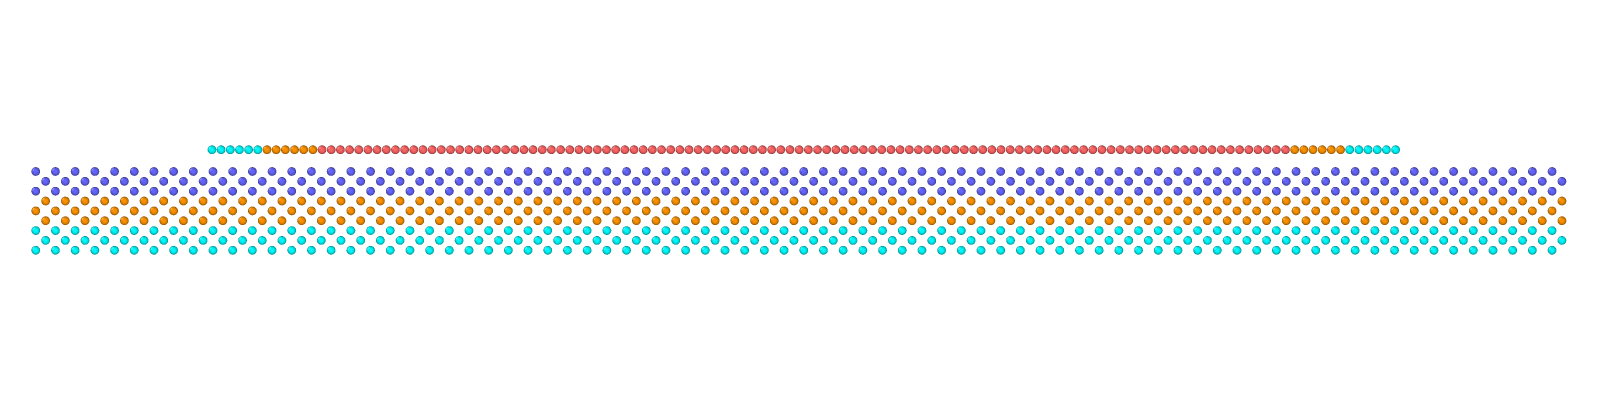
\includegraphics[width=\textwidth]{figures/system/system_sideview.png}
      \caption{Side view showing sheet on top of the substrate.}
      \label{fig:sideview}
  \end{subfigure}
  \hfill
  \begin{subfigure}[b]{0.80\textwidth}
      \centering
      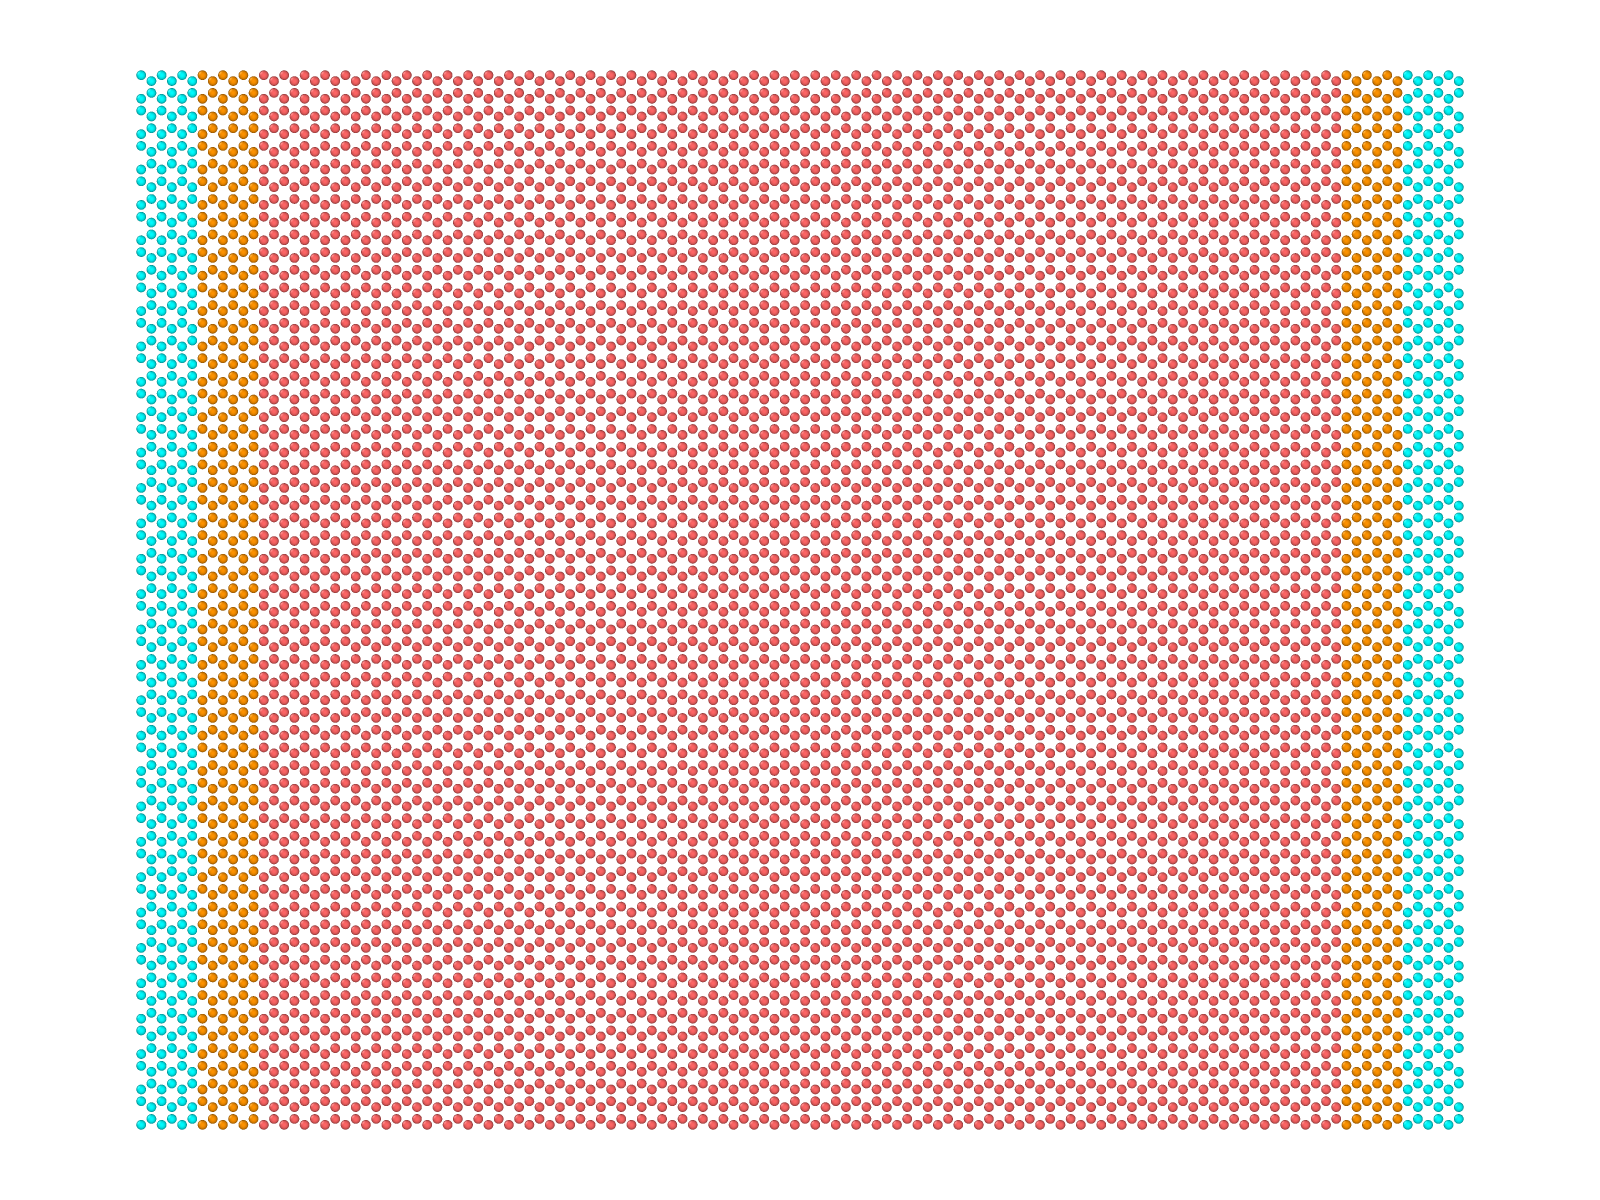
\includegraphics[width=\textwidth]{figures/system/system_topview.png}
      \caption{Top view showing only the sheet.}
      \label{fig:topview}
  \end{subfigure}
  \hfill
     \caption{System configuration colorized to indicate NVE parts (red), thermostat parts (green) and rigid parts (blue).}
     \label{fig:system}
\end{figure}

\begin{table}[H]
  \begin{center}
  \caption{Amount of atoms in the various system regions in the case of no cutting applied to the sheet.}
  \label{tab:system_count}
  \begin{tabular}{ |c|| c | c | c | c | c | c |} \hline
    \textbf{Region} & \textbf{Total}  & Sub region & Sub total & \textbf{NVE} &
    \textbf{NVT} & \textbf{Rigid} \\ \hline   
    \multirow{2}{*}{Sheet} & \multirow{2}{*}{7800} & Inner sheet & 6360 & 6360 &
    0 & 0 \\ %\hline
    & & Pull blocks & 1440 & 0 & 720 & 720 \\ \hline   
    \multirow{2}{*}{Substrate} & \multirow{2}{*}{19656} & Upper & 6552 & 6552 &
    0 & 0 \\ %\hline
    & & Middle & 6552 & 0 & 6552 & 0 \\ %\hline
    & & Bottom & 6552 & 0 & 0 & 6552 \\ \hline \hline   
    All & 27456 & \multicolumn{2}{r|}{} & 12912 & 7272 & 7272 \\ \hline 
  \end{tabular}
  \end{center}
\end{table}


\begin{table}[H]
  \begin{center}
  \caption{Sheet dimensions comparing the full sheet to its subdivisions: inner sheet and pull blocks.}
  \label{tab:sheet_dim}
  \begin{tabular}{ | l | r@{}l | r@{}l | c |} \hline
    \textbf{Group} & \multicolumn{2}{c|}{$x,y$-dim} & \multicolumn{2}{c|}{dim
    [Å]} & Area [Å$^2$]\\ \hline
  Full sheet & $x_S \: \times \: $ & $y_S$ &  $130.029 \: \times \:$ & $163.219$
  Å & $\phantom{2\times} 21,223.203$ \\ \hline
  Inner sheet & $x_S \: \times \:$ & $81.40 \ \%_{y_s}$ &  $130.029  \: \times
  \:$ & $132.853$ Å & $\phantom{2\times} 17,274.743$\\ \hline
  Pull blocks & $2 \times x_S \: \times \:$ & $ \phantom{0}9.30 \ \%_{y_s}$ & $2
  \times 130.029  \: \times \: $ & $\phantom{0}15.183$ Å  & $2 \times
  \phantom{0}1,974.230$ \\ \hline  
  \end{tabular}
  \end{center}
\end{table}


\section{Numerical procedure}
The numerical procedure related to the measurement of friction can be arranged
into the following steps. Some steps have been given a duration
denoted in parentheses in units of ps, \num{e-12} seconds.
\begin{enumerate}
  \item \textbf{Relaxation} (15 ps): The sheet and substrate are relaxed for 15 ps after being added in their crystaline form with a seperation distance of 3 Å which was found to be a reasonble estimate for the equilibrium distance at the temperature range of interest. The sheet is
  constrained under three hard spring forces, all with spring constant $10^5$
  eV/Å$^2$ $\sim$ \num{1.6e6} N/m: One spring attaches the sheet center of mass
  (\acrshort{CM}) to its orginal postion, preventing any drift. The
  remaining two springs are attatched the pull block ends, to their initial \acrshort{CM} position respectively, to prevent rotation. In principle, it would be sufficient to fixate just one of the ends in order to stop rotation, but we fixate both ends for the sake of symmetry. During the
  relaxtion phase the pull blocks are made rigid with respect to the z-direction
  only (perpendicular to the sheet). That is, all the forces in the z-direction
  is summed up and distributed on the pull blocks as a single external force, while it is free to expand and
  contract in the x-y-plane. This is mainly to ensure that it achieves the
  correct lattice spacing according to the temperature of the system. For the following phases the rigid parts of the pull block is in fact rigid with
  respect to all directions. The spring forces are terminated after the relaxtion phase. 
  \item \textbf{Stretch}: The sheet is stretched by seperating the two opposing rigid parts of the pullblock at constant velocity until the desired stretch amount is met. The duration of this phase is thus controlled by the  \textit{stretch speed} and \textit{stretch amount} parameters. 
  \item \textit{Pause} (5 ps): The sheet is relaxed for 5 ps after the stretch
  procedure to ensure that the sheet is stable and equilibrized after the applied stretch deformation. 
  \item \textbf{Normal load} (5 ps): The normal load is applied to the rigid
  parts of the pull blocks. Initially a viscous damping force, $F = -\gamma \vec{v}$, is added to the sheet to resist the rapid acceleraction of the sheet and prevent a hard impact between the sheet and substrate. The damping coefficient is set to $\gamma = \SI{8e-4}{nN/(m/s)}$ and terminated after 0.5 ps as this was visually found to be suitable for the extreme load cases of our intedned range of normal force. The remaining 4.5 ps devoted as a relaxtion phase. 
  \item \textbf{Sliding}: A virtuel atom is introduced into the simulation which
  exclusively interacts with the rigid parts of the pull through a spring force
  with variable spring constant $K$ in the x-y-plane. The z-direction is not
  affected by the spring force and is purely governed by the balance between normal load and the normal response from the sheet-substrate interaction. The
  virtual atom is immediately given a constant velocity, corresponding to a
  the \textit{sliding speed} parameter, which make the sliding force increase proportional to $\propto K(vt)^2$ for sliding speed $v$. An infinite sprig constant can also be choosen for which the spring is omitted and teh pull blocks are moved rigidly with the constant speed according to the sliding speed.
\end{enumerate}

In order to prevent rupturing, or detachment, of the sheet we monitor the nearest neighbours for each atom throughout the simularion. At the initial timestep the three nearest neighbours (at distance 1.42 Å) of all graphene atoms is recorded. If any of these nearest neighbours exceeds a threshold distance of 4
Å, indicating a bond breakage, this is marked as a rupture and we halt the simulation early. Thus, we ensure that no wear is allowed for the sheet. The substrate is way more robust and by running test simulation of high load and sliding speed we confirmed visually that no wear is accouring in the vicinity of the conditions used in the study

\section{Creating the sheet}

We are going to create a 2D sheet graphene sheet. 

\subsection{Graphene}
% (https://community.wvu.edu/~miholcomb/graphene.pdf)
% https://www.physics-in-a-nutshell.com/article/4/lattice-basis-and-crystal

Graphene is a single layer of carbon atom, graphite is the bulk, arranged in a
hexagonallattice structure. We can describe the 2D crystal structure in terms of
its primitive lattice vector and a basis. That is we populate each lattice site
by the given basis and translate it to fill the whole plane by any linear
combination of the lattice vectors
\begin{align*}
  \vec{T}_{mn} = m\vec{a_1} + n\vec{a_2}, \qquad m,n \in \mathbb{N}.
\end{align*}
For graphene we have the primitive lattice vectors 
\begin{align*}
  \vec{a_1} = a \left(\frac{\sqrt{3}}{2}, -\frac{1}{2}\right), \qquad \vec{a_2} = a \left(\frac{\sqrt{3}}{2}, \frac{1}{2}\right), \qquad |\vec{a_1}| = |\vec{a_2} = 2.46 \ \text{Å}.
\end{align*}
Notice that we deliberately excluded the third coordinate as we only consider a
single graphene layer on not the bulk graphite consisting of multiple layers
stacked on top of each other. The basis is 
\begin{align*}
  \Big\{\Big(0,0\Big), \frac{a}{2}\Big(\frac{1}{\sqrt{3}}, 1 \Big) \Big\}
\end{align*}
It turns out that the spacing between atoms is equal for all paris with an
interatomic distance 
\begin{align*}
  \left|\frac{a}{2}\Big(\frac{1}{\sqrt{3}}, 1 \Big)\right| \approx 1.42 \ \text{Å}.
\end{align*}


\begin{figure}[H]
  \centering
  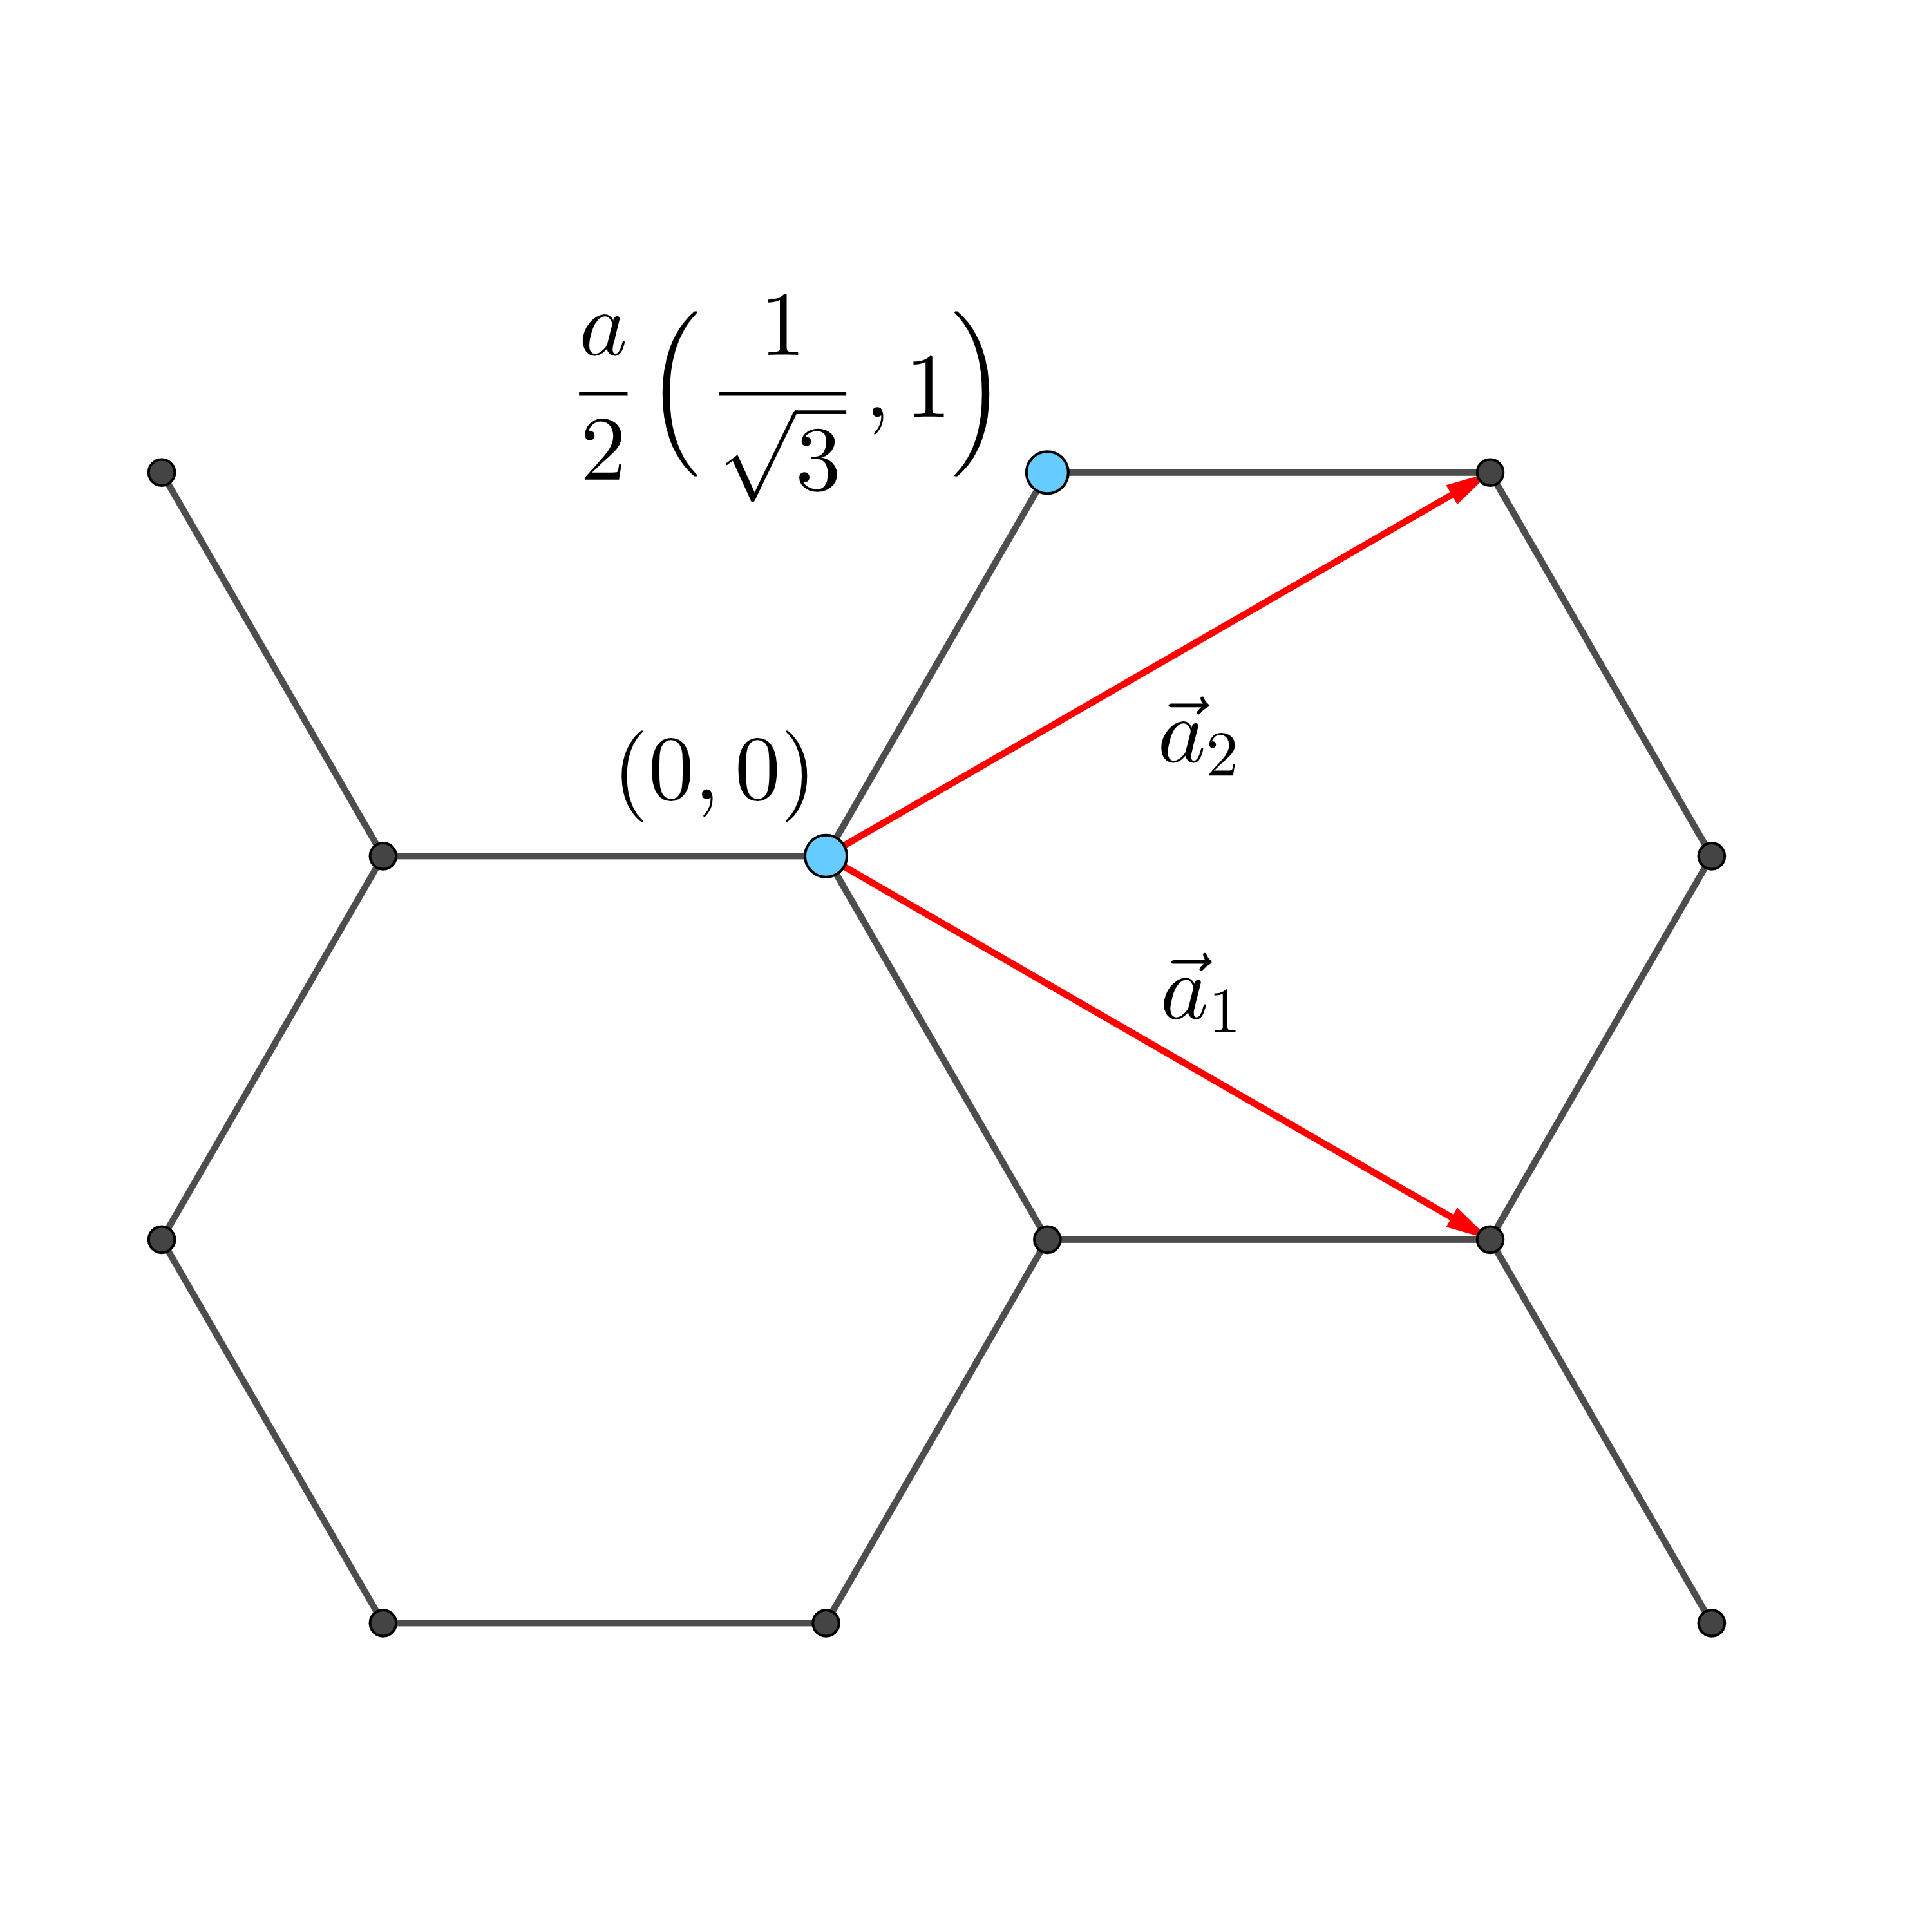
\includegraphics[width=0.3\linewidth]{figures/system/crystal.png}
  \caption{Graphene crystal structure with basis.}
  \label{fig:graphene_crystal}
\end{figure}



\subsection{Indexing}
In order to define the cut patterns applied to the graphene sheet we need to
define an indexing system. We must ensure that this gives an unique description
of the atoms as we eventually want to pass a binary matrix, containing 0 for
removed atoms and 1 for present atoms, that uniquely describes the sheet. We do
this by letting the x-coordinate point to zigzag chains and the y-coordinate to
the position along that chain. This is illustrated in figure
\cref{fig:atom_indexing}. Other solutions might naturally invole the lattice
vectors, but as these are used to translate between similar basis atoms
unfortunate duality is introduced as one need to include the basis atom of
choice into the indexing system. Additionally, we want a system where the
indexes reflect the relative physical position of neighbours . That is, atom
$(i, j)$ is in the proximity of $\{(i+1, j), (i-1, j), (i, j+1), (i, j-1)\}$.
However, only three of them is categorized as nearest neighbours due to the
hexgonal structure of the lattice. While $(i, j\pm 1)$ is always a nearest
neighbour the neighbour in the x-direction flip sides when incrementing either
x- or y-coordinate. That is the nearest neighbours (NN) is decided as
\begin{equation}
  \begin{aligned}
    (i + j) \ \text{is even} &\rightarrow \text{NN} = \{(i-1, j), (i, j+1), (i, j-1)\}, \\
    (i + j) \ \text{is odd} &\rightarrow \text{NN} = \{(i+1, j), (i, j+1), (i, j-1)\}.
  \end{aligned}
  \label{eq:atom_neigh_idx}
\end{equation}


\begin{figure}[H]
  \centering
  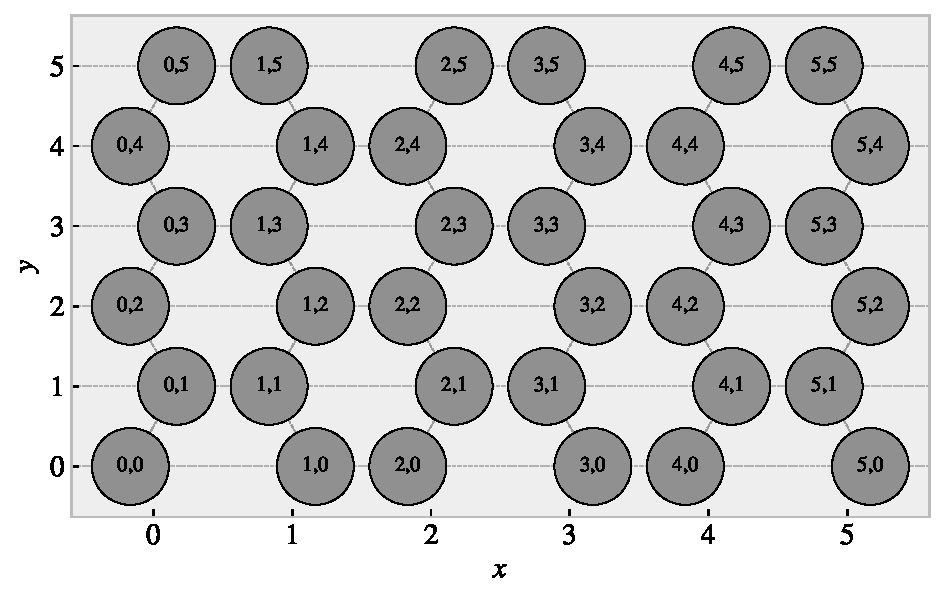
\includegraphics[width=0.7\linewidth]{figures/system/atom_indexing.pdf}
  \caption{Graphene atom indexing}
  \label{fig:atom_indexing}
\end{figure}



\subsection{Removing atoms}

As a mean to ease the formulation of cut patterns we introduce pseudo center
element in each gap of the hexagonal honeycombs, see figure
\cref{fig:center_indexing}. 

\begin{figure}[H]
  \centering
  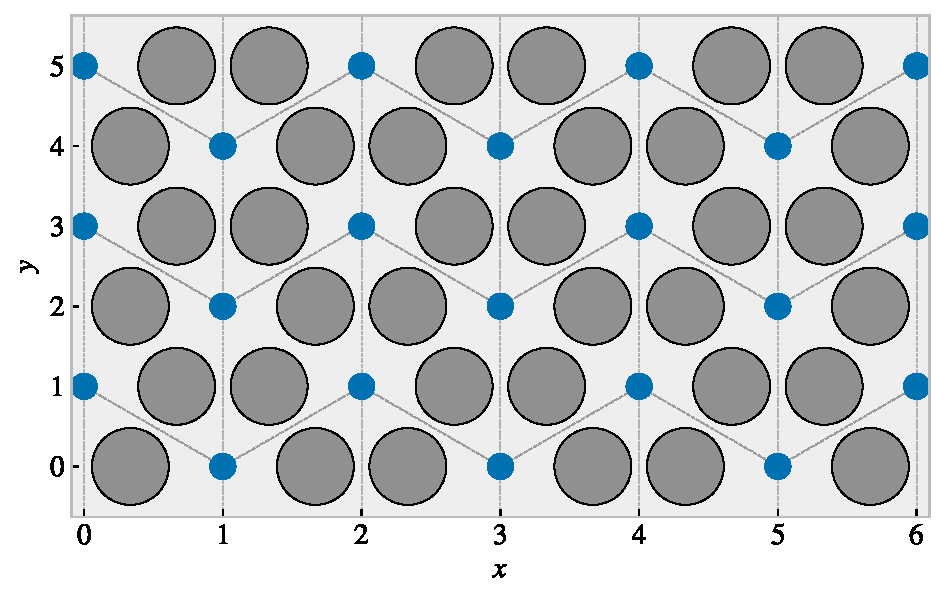
\includegraphics[width=0.7\linewidth]{figures/system/center_indexing.pdf}
  \caption{Graphene center indexing}
  \label{fig:center_indexing}
\end{figure}


Similar to the case of the indexing for the carbon atoms themselves the nearest
neighbour center elements alternate with position, this time only along the
x-coordinate index. Each center element has six nearest neighbours, in clock wise
direction we can denote them: ``up'', ``upper right'', ``lower right'',
``down'', ``lower left'', ``upper left''. The ``up'' and ``down'' is always
accesed as $(i,j\pm 1)$, but for even $i$ the $(i+1,j)$ index corresponds to the
``lower right'' neighbour while for odd $i$ this corresponds to the ``upper
right'' neighbour. This shifting applies for all left or right neighbours and
the full neighbour list is illustrated in \cref{fig:center_directions}. 


\begin{figure}[H]
  \centering
  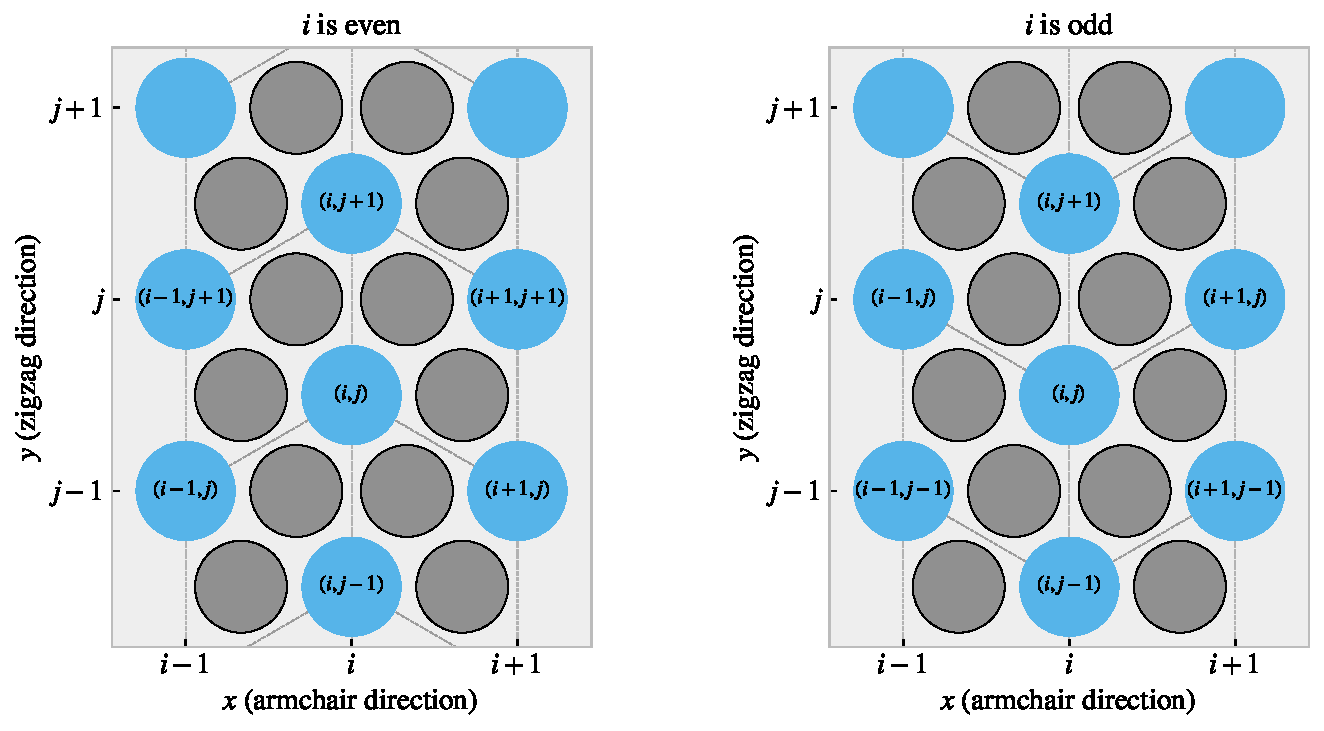
\includegraphics[width=0.7\linewidth]{figures/system/center_directions.pdf}
  \caption{Graphene center elements directions}
  \label{fig:center_directions}
\end{figure}


We define a cut pattern by connecting center elements into connected paths. As
we walk element to element we remove atoms according to one of two rules 
\begin{enumerate}
  \item Remove intersection atoms: We remove the pair of atoms placed directly
  in the path we are walking. That is, when jumnping to the ``up'' center
  element we remove the two upper atoms located in the local hexagon of atoms.
  This method is sensitive to the order of the center elements in the path. 
  \item Remove all surrounding atoms: We simply remove all atoms in the local
  hexagon surrounding each center element. This method is indepdent of the
  ordering of center elements in the path.
\end{enumerate}

We notice that removing atoms using either of these rules will not garuantee an
unique cut pattern. Rule 1 is the more sensitive to paths but we realize that,
for an even $i$, we will remove the same five atoms following either of the
following paths.
\begin{align*}
  (i, j) &\rightarrow \underbrace{(i+1,j+1)}_{\text{upper right}} \rightarrow \underbrace{(i, j+1)}_{\text{up}} \rightarrow \underbrace{(i+1, j+2)}_{\text{upperright + up}} \rightarrow \underbrace{(i+1, j+1)}_{\text{upper right}} \\
  (i, j) &\rightarrow \underbrace{(i+1,j+1)}_{\text{upper right}} \rightarrow \underbrace{(i+1, j+2)}_{\text{upperright + up}} \rightarrow \underbrace{(i, j+1)}_{\text{up}}
\end{align*}

For rule 2 it is even more abovious that different paths can result in the same
atoms being removed. This is the reason that we needed to define and indexing
system for the atom position itself even though that all cuts generated manually
will use the center element path as reference. \\

Illustrate some delete path?



\section{Kirigami patterns}

We propose a series of kirigami inspired cut patterns for the altering of the graphene sheet. We seek inspiration from macroscale patterns that showcases a considerable amount of out of plane buckling when stretched. We choose to imitate two different designs: 1$)$ An alternating repeating series of perpendicular cuts as shown in \cref{fig:kirigami_inspiration_a} commonly used in studies of morphable metematerials \cite{new_pop_up}. This patteren produce surface buckling with a tetrahedron (three sided pyramid) shape when stretched. 2$)$ A more intricate pattern shown in \cref{fig:kirigami_inspiration_b} which is used Scotch\textsuperscript{TM} Cushion Lock\textsuperscript{TM} \cite{cushion_wrap} as protective wrap for items during shipping. This pattern buckles into a hexagoal honeycomb structure when stretched. In addition to the modeling of the so-called \textit{tetrahedron} and \textit{honeycomb} patterns we also create a series of random walk styled cut patterns.


\begin{figure}[H]
  \centering
  \begin{subfigure}[t]{0.48\textwidth}
      \centering
      \includegraphics[width=\textwidth]{figures/system/pop_up_inspiration.png}
      \caption{}
      \label{fig:kirigami_inspiration_a}
    \end{subfigure}
    \hfill
    \begin{subfigure}[t]{0.48\textwidth}
      \centering
      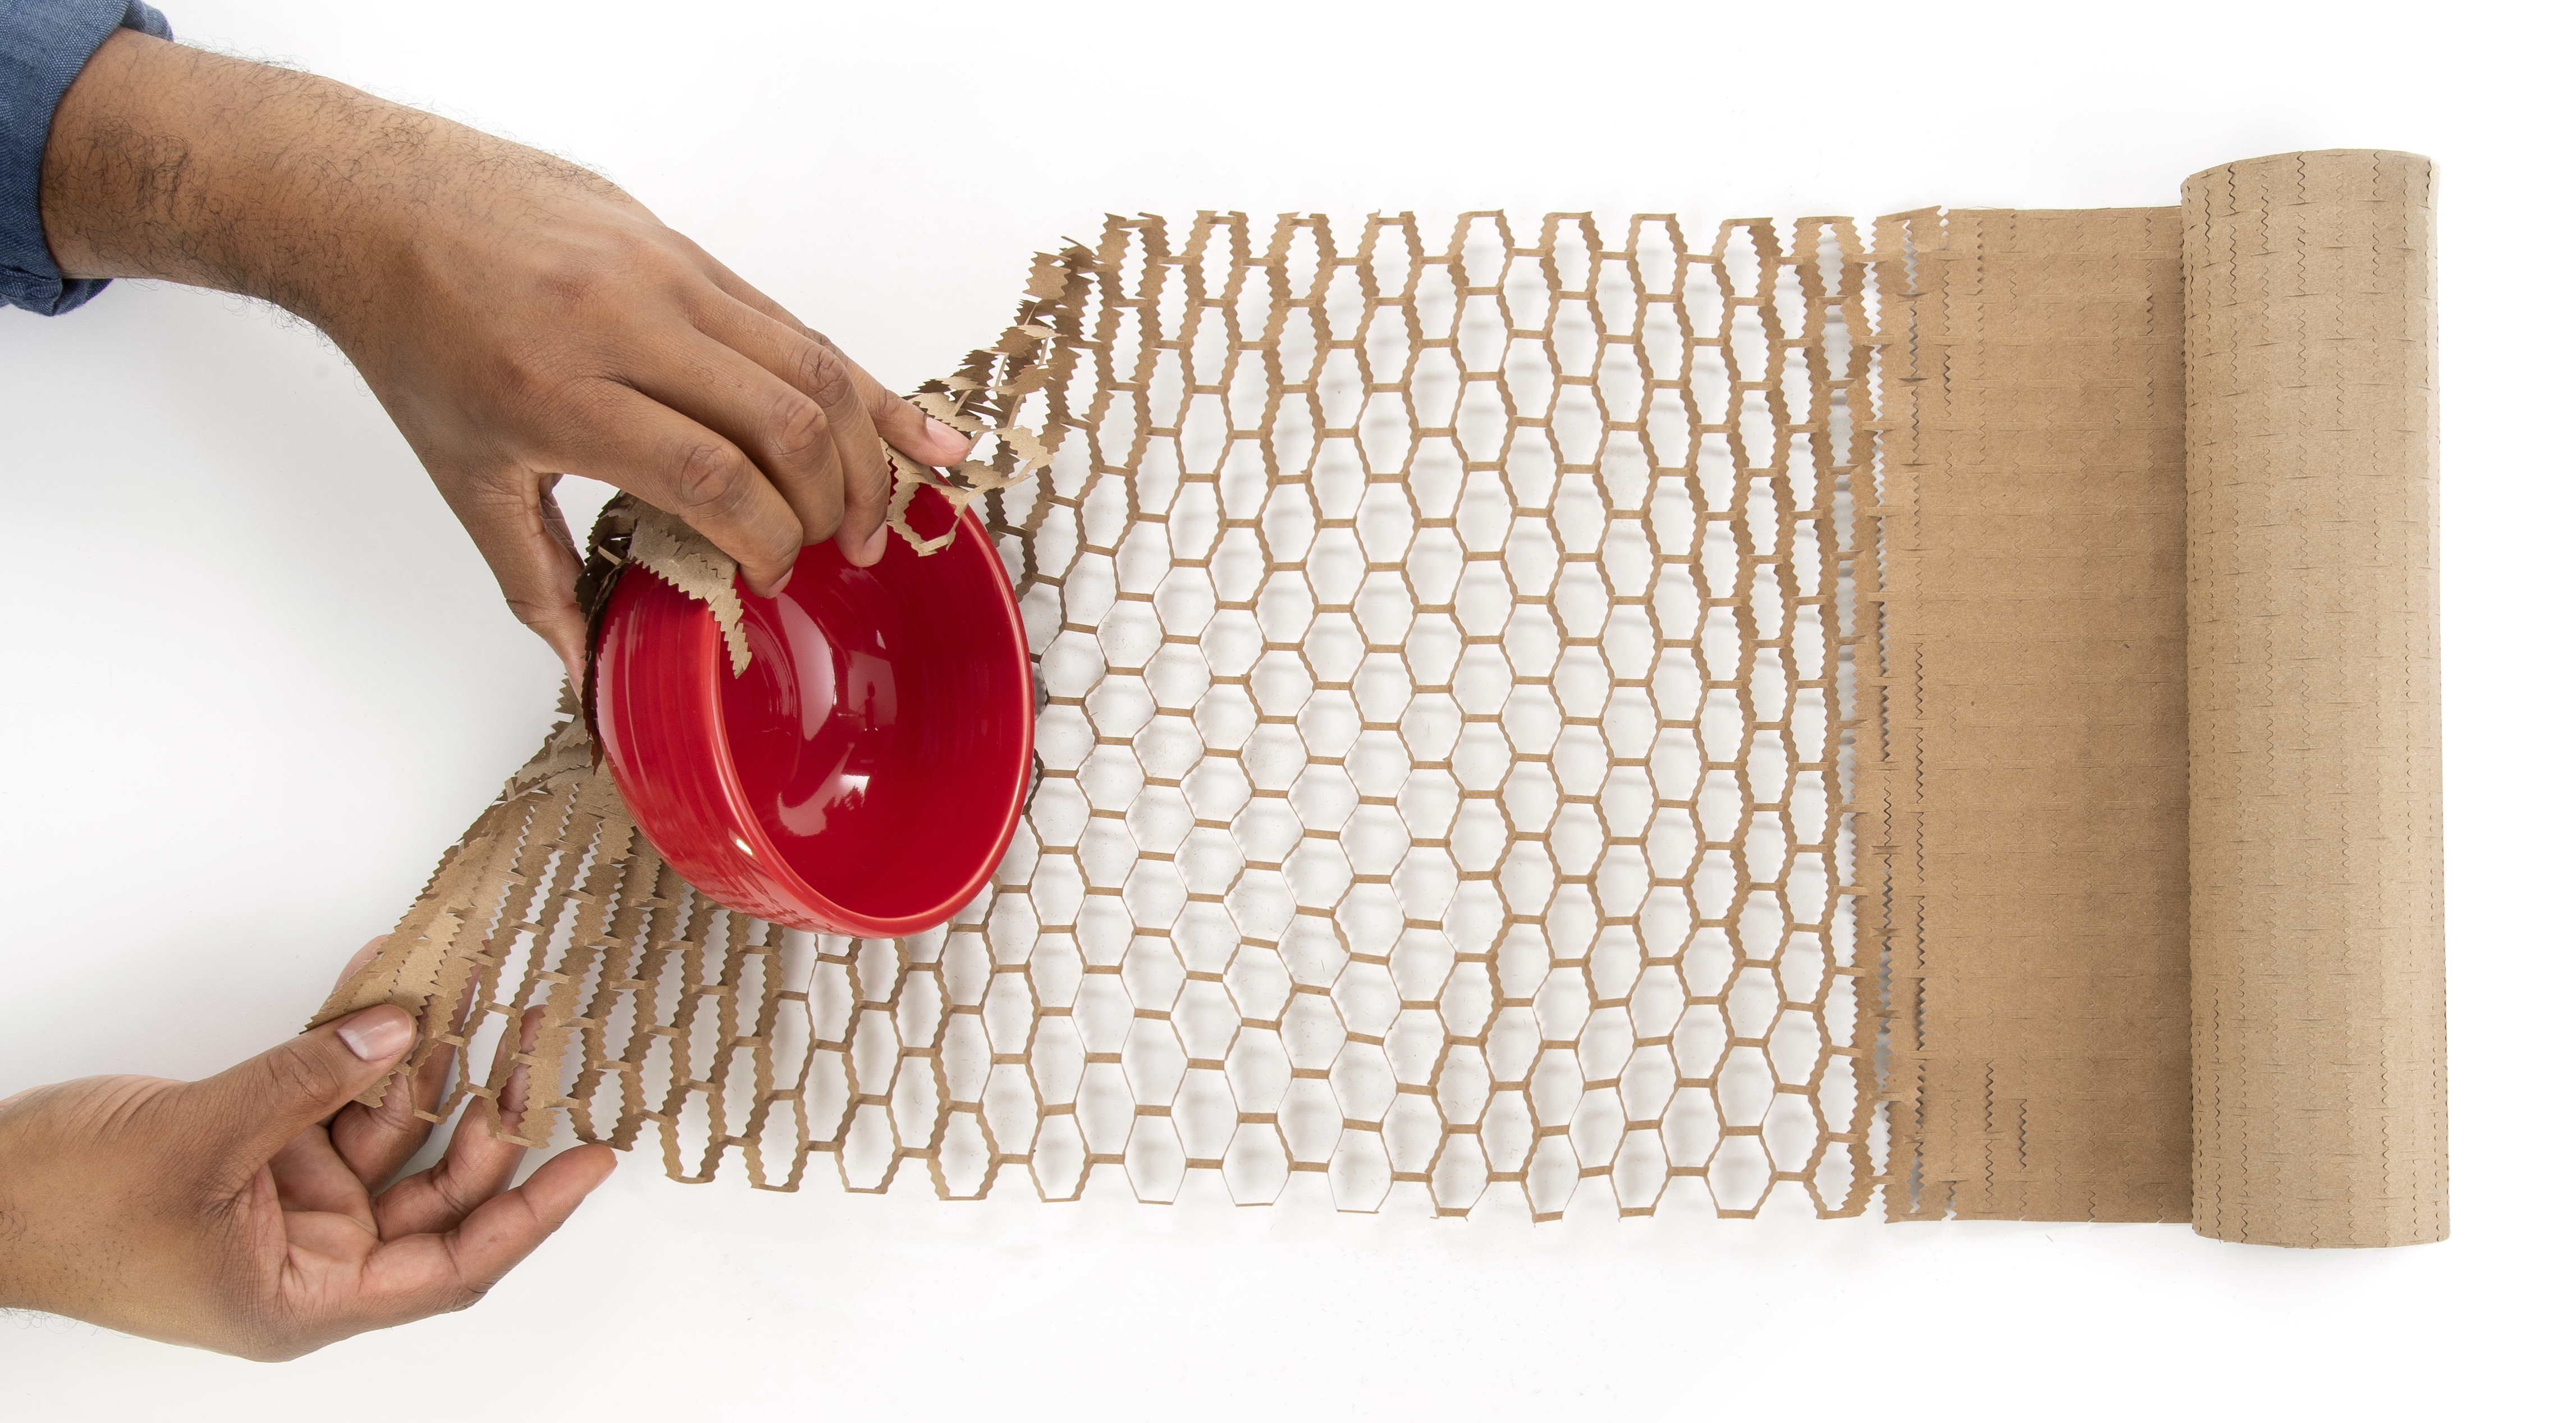
\includegraphics[width=\textwidth]{figures/system/honeycomb_inspiration.jpg}
      \caption{}
      \label{fig:kirigami_inspiration_b}
  \end{subfigure}
  \hfill
     \caption{Macroscale kirigami cut patterns used as inspiraton for the nanoscale implementation. (a) Alternating perpendicular cuts producing a tetrahedron shaped surface buckling when stretched \cite{new_pop_up}. (b) Scotch\textsuperscript{TM} Cushion Lock\textsuperscript{TM} \cite{cushion_wrap} producing a honeycomb shaped surface buckling when stretched.}
     \label{fig:kirigami_inspiration}
\end{figure}

\subsection{Tetrahedron}
The \textit{tetrahedron} pattern is defined in terms of center elements for which all
atoms sourrounding a given center element are removed. The pattern is
characterized by two straight cuts, here denoted line 1 and line 2, arranged
perpendicular to each other such that one line aligns with the center of the
other line and with a given spacing in between. In order to achieve
perpendicular cuts we cannot rely purely on the six principal directions
corresponding to the center element neighbours which is spaced by 60$^\circ$.
Instead, we let line 1 run along the center elemnts in the direction of the
``upper right'' center elements (and ``lower left'') while line 2 goes in the
direction between the ``lower'' and ``lower right'' center elements
corresponding to the direction $(1/\sqrt{3}, -1)$. We define variations of the
pattern by the number of center elements $L_1$ and $L_2$ in line 1 and 2
respectively together with the spacing between the lines $d$ as the tuple $(L_1,
L_2, d)$. The pattern is constructed by translating the two lines to thew whole sheet while according to the spacing. Due to the alignment criterias of having one line point to the center of the other line we can only have odd line length to have a clearly defined center element in the center of each line. Furthermore, in order to ensure that each translated center element stays on the same odd or even type center element we must in practice require that $|L_2 - L_1| = 2, 6, 10, \cdots$. In \cref{fig:pop_up} we see a visual representation of the pattern components for the $(7, 5, 2)$ patteren. 


\begin{figure}[H]
  \centering
  \begin{subfigure}[t]{0.48\textwidth}
      \centering
      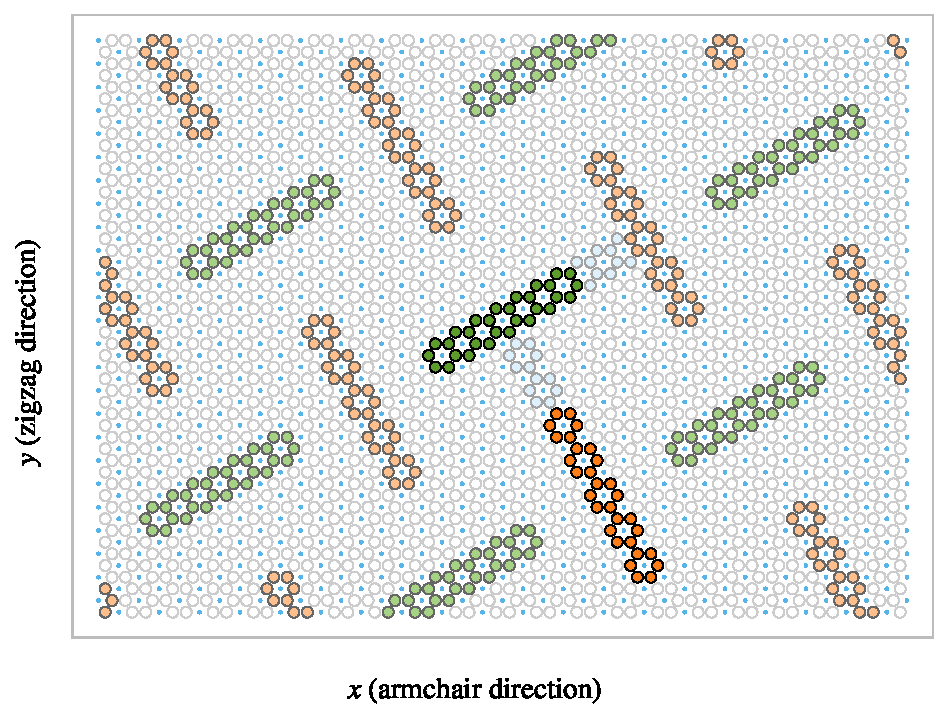
\includegraphics[width=\textwidth]{figures/system/pop_up_inverse.pdf}
      \caption{}
      \label{fig:pop_up_a}
    \end{subfigure}
    \hfill
    \begin{subfigure}[t]{0.48\textwidth}
      \centering
      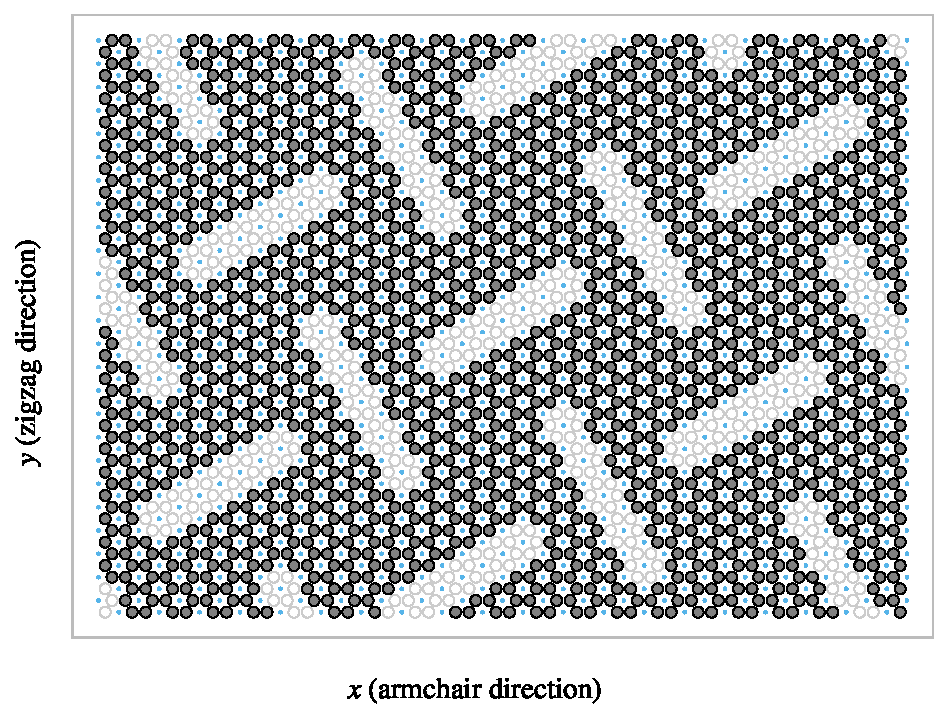
\includegraphics[width=\textwidth]{figures/system/pop_up_pattern.pdf}
      \caption{}
      \label{fig:pop_up_b}
  \end{subfigure}
  \hfill
     \caption{Visual representation of the tetrahedron pattern consisting of two perpendicular lines, line 1 and line 2, of length $L_1$ and $L_2$ respectively with spacing $d$. This example used $(L_1, L_2, d) = (7, 5, 2)$. $(a)$ Highlight of the atoms removed. Line 1 is shown in green and line 2 in orange, with lighter colors for the translated variations, and the spacing is shown in light blue. $(b)$ The sheet after applying the cut pattern where the grey circles denote atoms and the transparent white denotes removed atoms. The small blue circles show the center elements for reference}.
     \label{fig:pop_up}
\end{figure}

In addition to the three parameters $L_1, L_2, d$, the pattern is also anchored to a reference point which describes the position of line 1 and 2 before translating to the whole sheet. Due to the repeating structure of the pattern there exist a small finite number of unique reference positions. For the pattern $(7, 5, 2)$ used as an example in \cref{fig:pop_up} there are 140 \footnote{The calculation of this is rather complicated in comparision of the importance in this context. Thus, we exclude the formula for this calculation as the derivation is rather handwavy and the number stated here is numerically backed for this specific parameter set.} Some additional variation of the pattern deviaiton from the example in \cref{fig:pop_up} is showcased in \cref{fig:pop_up_flavors}

\begin{figure}[H]
  \centering
  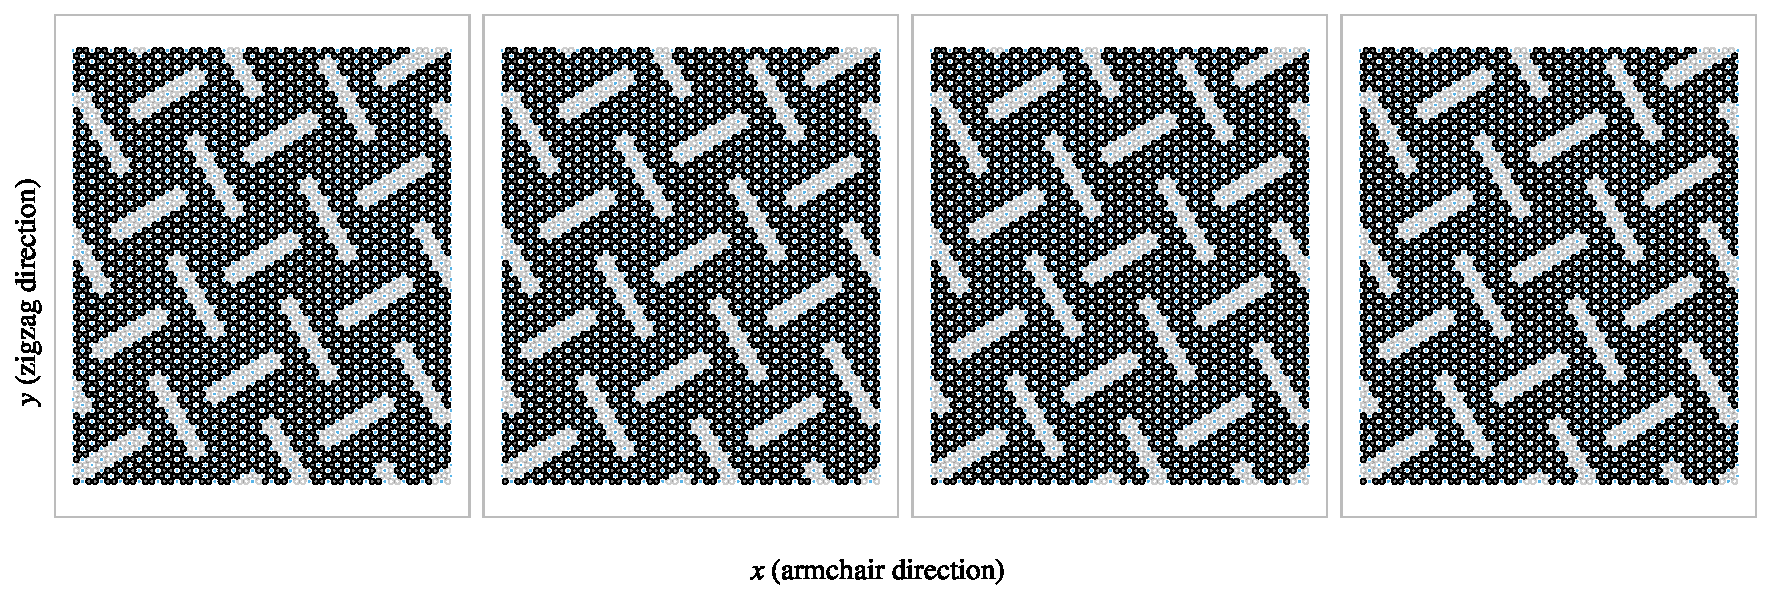
\includegraphics[width=\linewidth]{figures/system/pop_up_flavors.pdf}
  \caption{}
  \label{fig:pop_up_flavors}
\end{figure}



\subsection{Honeycomb}
The \textit{honeycomb} pattern is defined, similarly to the tetrahedron pattern,
in terms of center elements for which all atoms sourrounding a given center
element are removed. The honeycomb pattern is build from a repeating series of
cuts remniscient of a roman numeral one put on its side
(\rotatebox[origin=c]{90}{\MakeUppercase{\romannumeral 1}}). With a given spacing these are put next to each other in the x-direction (\rotatebox[origin=c]{90}{\MakeUppercase{\romannumeral 1}}
\rotatebox[origin=c]{90}{\MakeUppercase{\romannumeral 1}}
\rotatebox[origin=c]{90}{\MakeUppercase{\romannumeral 1}}) to achieve a row
where only a thin \textit{bridge} in between each cut is left to connect the sheet in the y-direction. By placing multiple rows along the y-direction with alternating x-offsett we get the class of honeycomb patterns as visualized in \cref{fig:honeycomb}. The pattern
is described in terms of the parameters: (x-width, y-width, bridge thickness,
bridge length) which is annotated in \cref{fig:honeycomb_a} where the parameters (2, 2, 1, 5) is used as an example. Some additional variations of the pattern class is showcased in \cref{fig:honeycomb_flavors}


\begin{figure}[H]
  \centering
  \begin{subfigure}[t]{0.48\textwidth}
      \centering
      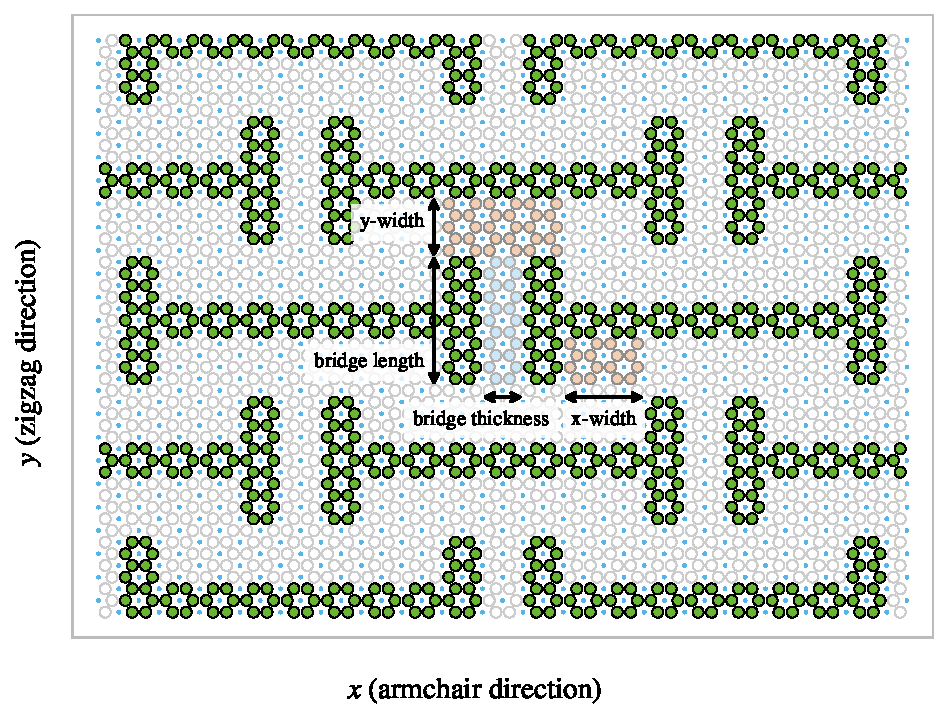
\includegraphics[width=\textwidth]{figures/system/honeycomb_inverse.pdf}
      \caption{}
      \label{fig:honeycomb_a}
    \end{subfigure}
    \hfill
    \begin{subfigure}[t]{0.48\textwidth}
      \centering
      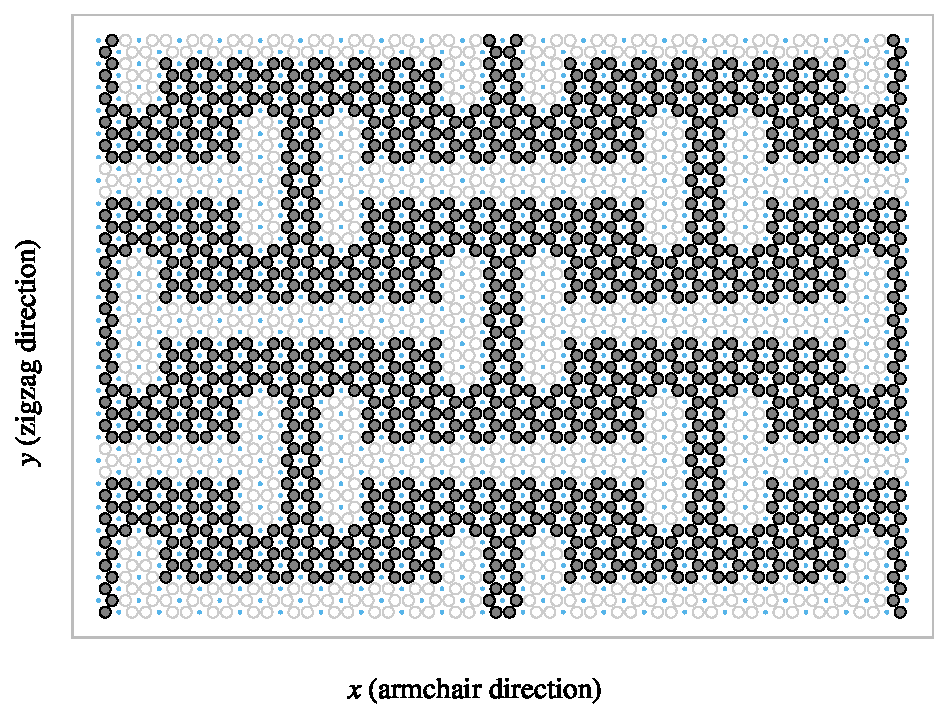
\includegraphics[width=\textwidth]{figures/system/honeycomb_pattern.pdf}
      \caption{}
      \label{fig:honeycomb_b}
  \end{subfigure}
  \hfill
     \caption{}
     \label{fig:honeycomb}
\end{figure}


\begin{figure}[H]
  \centering
  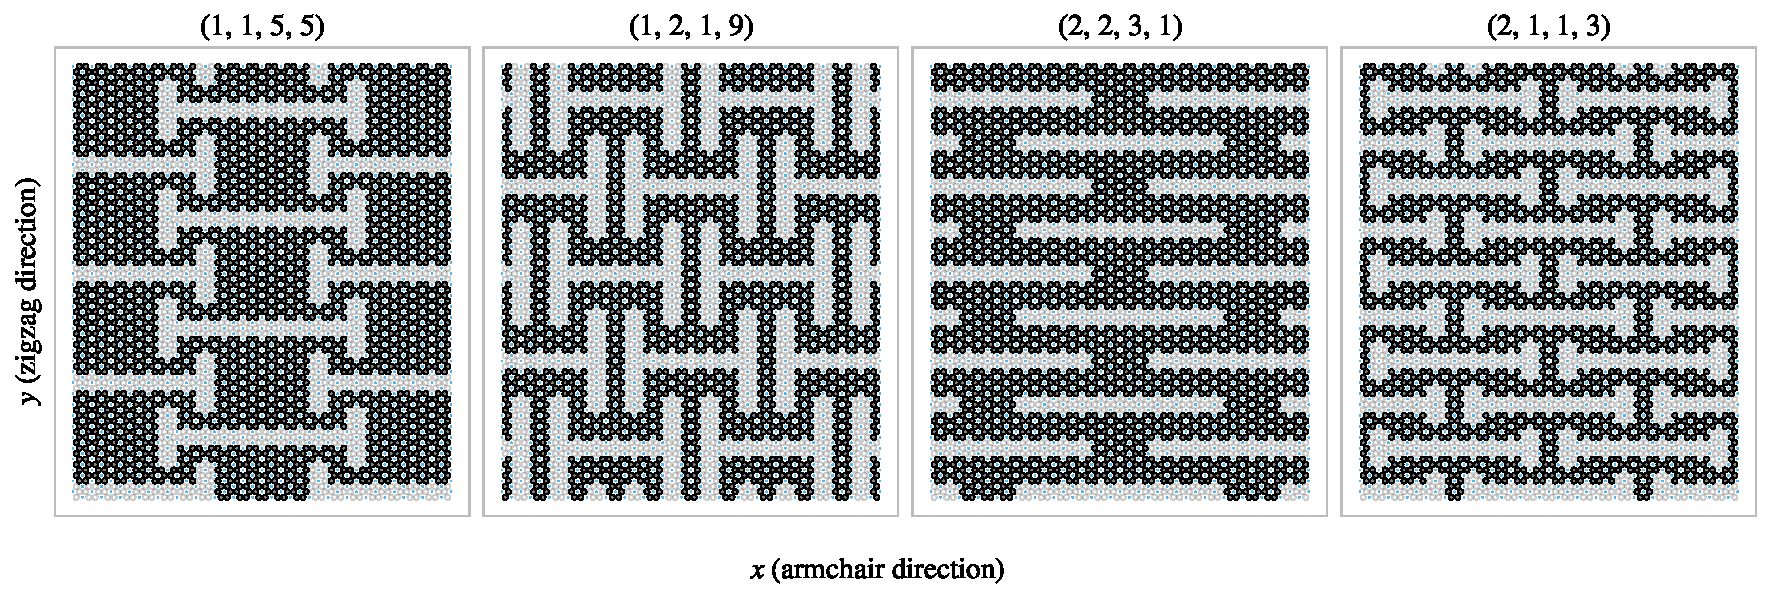
\includegraphics[width=\linewidth]{figures/system/honeycomb_flavors.pdf}
  \caption{}
  \label{fig:honeycomb_flavors}
\end{figure}




\subsection{Random walk}
The random walk serves as a method for introducing random patterns into the dataset with the scope of populating the configuration space more broadly than achieved with the more systematic patterns classes described above. By this argument a more straightforward way to create random configurations could be achieved by random noise, either uniform or gaussian. However, this would often leave the sheet detached with lots of non-connected atom clusters, and intuitively we do not find this promising for the generation of large scale organized structures which is hypothesized to be of interest. The random walk pattern generation is characterized by the parameters summarized in \cref{tab:RW_params} which will be introduced throughout the following paragraphs. 


\begin{table}[H]
  \begin{center}
  \caption{Parameters for the random walk generator.}
  \label{tab:RW_params}
  \begin{tabular}{ | c | c | m{8cm} |} \hline
  \textbf{Parameters} & \textbf{Value} & \textbf{Description}  \\ \hline
  Num.\ walkers ($M$) & Integer $\ge$ 1 & Number of random walks to be initiated on the sheet (one at a time). \\ \hline
  Max.\ steps ($S$)  & Integer $\ge$ 1 &The maximum steps allowed for any random walker. \\ \hline
  Min.\ distance  & Integer $\ge$ 0 &The minimum distance required between any future paths and the previous paths in terms of the least walking steps in between. \\ \hline
  Bias  & Vector & Bias direction and strength defining the discrete probability for the chocie of the next site. \\ \hline
  Connection  & Atoms / Center elements & Walk between atoms or between center elements (removing all adjecent atoms). \\ \hline
  Avoid unvalid  & True/False & Whether to remove already visited sites from the neighbour list before picking the next site. This prevents jumping to already visited site and lowers the likelihood of early termination.  \\ \hline
  Stay or break  & $p = [0,1]$ & \\ \hline
  Periodic  & True/False & Whether to use periodic boundary conditions of all four sides. \\ \hline
  Avoid clustering  & Integer $\ge$ 0 & Amount of times to retry random walk in order to avoid detached clusters. Non-spanning clusters are removed after this amount of tries.\\ \hline
  RN6  & True/False & Randomly change the bias direction between one of the six center element directiosn for each random walker deployed. \\ \hline
  Grid start  & True/False & The option to have the random walkers start in an evenly spaced grid. \\ \hline
  Centering  & True/False & Relocate the path of a random walk after termination such that the path center of mass gets closer to the starting point (without violating the rules for travelling on already visited sites).\\ \hline
  \end{tabular}
  \end{center}
\end{table}

\subsubsection{Fundamentals} % M, S, Connection, Periodic, Avoid unvalid
For an uncut sheet we deploy $M$ random walkers one at a time and let them walk
for a maximum number of $S$ steps. We can either let the walker travel between
atom sites, removing the atoms in the path as it goes, or between center
elements, removing all sourrounding atoms - \textit{Connection: Atom/Center
elements}. Nonetheless, we will always remove a site once visited such that the
walker itself or any other walker cannot use this site again. This corresponds
with the property of a self avoiding random walk, but it futhermore constraint
the walkers not to visit any path previously visited by another walker on the
sheet. By default, the walker has an equal chance of chosing any of its adjecent
neighbours for the next step, i.e.\ we draw the next step from a discrete
uniform distribution. Optionally we can use periodic bounary conditions,
\textit{Periodic: True/False}, allowing neighbouring sites to be connected
through the edge in both the x and y-direction. When traveling on atom sites
this gives three nieghbour options for the next step while traveling on the
center elements gives six neighbour options. If the walker happens to arrive at
an already visited site the walk is terminated early. Optionally, we can choose
to remove any neighbouring sites already visited from the neighbour list,
\textit{Avoid unvalid: True/False}, and choose uniformly between the remaining
options instead. This prolongs the walking distance. However, the walker is
still able to find itself in a situation where no neighbouring sites is
availble, note that it cannot backtrack its own path either, and in such a case
the walk is always terminated dispite the setting of \textit{Avoid unvalid}.


\subsubsection{Spacing of walking paths} % minimum distance
In order to control the spacing between the paths of the various walkers we
implement a so-called \textit{minimum distance: 0, 1, \ldots} parameter,
describing the spacing required between paths in terms of the least amount of
steps. When a walker has ended its walk, either by early termination or hitting
the maximum limits of steps, all sites within a walking distance of the minimum
distance is marked as visited, allthough they are not removed from the sheet.
This prevents any subsequent walkers to visit those sites in their walk
according to the general behaviour described in the
previous paragraph. In practice this is done through a recursive algorithm as described in algorithm \cref{algo:walk_dis}. For a given path the function walk\_distance() is called with the input being a list of all sites in the given paths. The function will then for each site gather all site neighbours (regardless of their state on the sheet) and call itself using this neighbour list as input while incrementing a distance counter passed along. This will result in an expansion along all possible outgoing paths from the initial path of interest which is terminated when the distance counter hits the minimum distance limit. The function will then return the final neighbour lists which is cummulated into a final output corresponding to a list of all sites within the minimum distance to the path.

\begin{algorithm}[H]
  \caption{Recursive algorithm implemented as class method to mark sites within a distance of the class attribute self.min\_dis.}
  \label{algo:walk_dis}
  \begin{algorithmic}[1]
    \Require self.min\_dis $>$ 0 \Comment{This pseudocode does not handle other cases}
    \Function{walk\_distance}{self, input, dis = 0, pre = [ ]}
      % \State neigh $\gets$ NewList() 
      \State new\_neigh $\gets$ [ ] \Comment{Initialize list for new neighbours}
      \For{site in input}
        \State neigh $\gets$ get\_neighbouring\_sites(site) \Comment{Get sourrounding neighbours}
        \For{n in neigh}
          \If {(n not in pre) and (n not in new\_neigh)} \Comment{If not already added}
            \State AddItem(new\_neigh, n)
          \EndIf
        \EndFor
      \EndFor
      \State dis += 1 \Comment{Increment distance counter}
      \If{dis $\ge$ self.min\_dis} \Comment{Max limit hit}
        \State \Return input + new\_neigh 
      \Else \Comment{Start a new walk from each of the neighbouring sites}
        \State pre $\gets$ input
        \State \Return pre +  self.walk\_distance(new\_neigh, dis, pre)
      \EndIf
    \EndFunction
  \end{algorithmic}
\end{algorithm}


% Show figure of the self.visited shadowing  ???

\subsubsection{Bias} % Bias
We include the option perform biased random walk through the \text{Bias:
(direction, strength)} parameter option. We implement this by modelling each
walking step as an analog to the canonical ensemble under the influence of an
external force $\vec{F}$ representing the bias. For such a system each
microstate $i$, corresponding to the sites in the neighbour list, has the
associated probability $p_i$ given by the Gibbs–Boltzmann distribution
\begin{align*}
  p_{i} = \frac{1}{Z}e^{-\beta E_i}, \qquad Z = \sum_i e^{-\beta E_i},
\end{align*}
where $Z$ is the canonical partition function, $\beta = 1/k_B T$ for the
boltzmann constant $k_B$ and temperature $T$, and $E_i$ the energy of site $i$.
We model the energy of each site as the work required to move there. For a step
$\vec{s}$ the energy becomes $E_i = -\vec{s}\cdot\vec{F}$, where we notice that
the energy is negative for alligned bias and step analogous to an energy gain by
moving there. Due to the symmetry of both the atom sites and the center elements
sites the step length to neighbouring sites will always be equal. By defining
the bias magnitude $B = \beta|\vec{F}||\vec{s}|$ we get that the probability for
jumping to site $i$ is given by
\begin{align*}
  p_i = \frac{1}{Z}e^{B\hat{\vec{s}}\cdot\hat{\vec{F}}} \propto e^{B\hat{\vec{s}}\cdot\hat{\vec{F}}},
\end{align*}
 where the hat denotes the unit direction of the vector. The bias magnitude $B$
 captures the opposing effects of the magnitude of the external force and the
 temperature of the system as $B\propto |\vec{F}|/T$. We notice that
 $\hat{\vec{s}}\cdot\hat{\vec{F}} = \cos{(\theta)}$ for the angle $\theta$
 between the step and bias direction. This shows that the bias will have the
 biggest positive contribution when the step direction is allinged with the bias
 direction ($\theta = 0$), have no contribution for orthogonal directions
 ($\theta = \pm \pi/2$) and biggest positive contribution when the directions
 are antiparallel ($\theta = \pi$). The partition function serves simply as a
 normalization constant which in practice is  excluded ($Z = 1$) from the
 calculation of $p_i$ initially and then enforced at the final stage as a
 divition by the sum of all $p_i$. In the numerical implementation we then pick
 the step destination weighted by the discrete probability distribtion $p_i$. In
 \cref{fig:bias_prob} we have illustrated how a bias of different strength impacts the probability disitrbution for a random walk between center elements. We can visually confirm that the bias will favorise the directions that lies closes to the bias direction. This favorization is more distinct at high bias strenghs while at low strength $B\to0$ we get a uniform distribution whichi alligns with the default unbiased random walk. 


\begin{figure}[H]
  \centering
  \begin{subfigure}[t]{0.48\textwidth}
      \centering
      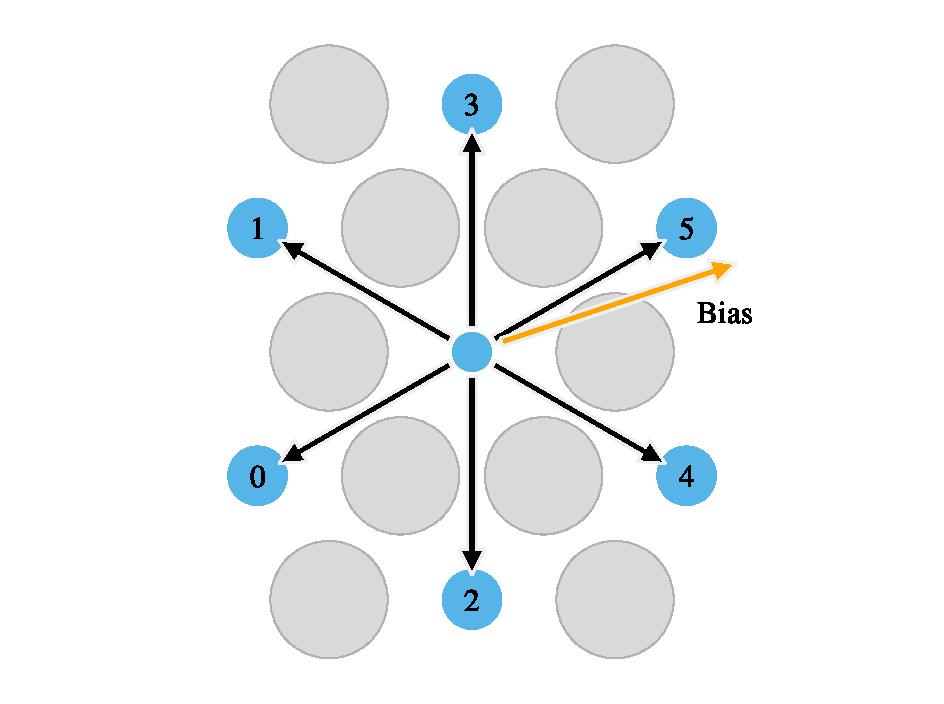
\includegraphics[width=\textwidth]{figures/system/bias_prob_a.pdf}
      \caption{}
      \label{fig:bias_prob_a}
    \end{subfigure}
    \hfill
    \begin{subfigure}[t]{0.48\textwidth}
      \centering
      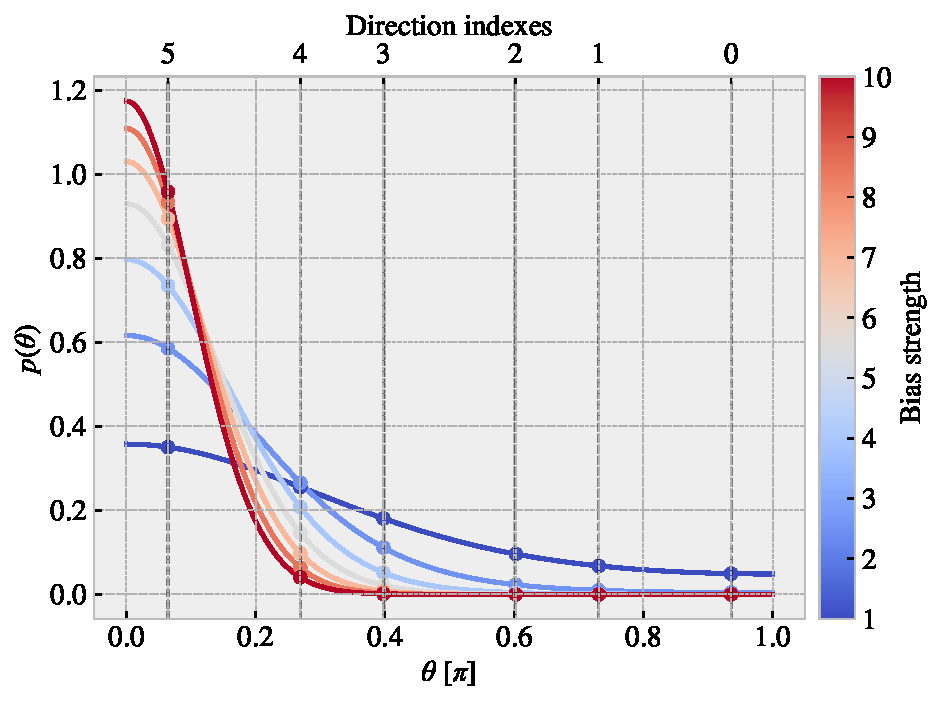
\includegraphics[width=\textwidth]{figures/system/bias_prob_b.pdf}
      \caption{}
      \label{fig:bias_prob_b}
  \end{subfigure}
  \hfill
     \caption{Illustration of the probability distribution for the various step direction during a bias random walked between center elements. $(a)$ Shows the possible step directions as black arrows pointing towards the neighbouring center elements shown as blue circles. The bias direction is denoted as an orange arrow and the numbering indicates the most likely direction to take (1) towards the least likely (6). The atoms sites are marked as grey circles for reference. $(b)$ The probability distribution as a function of angle between the direction of choice and the bias direction. The disitrbution is normalized according to the discrete probabilities marked with dots for which the continous line simple highlights the curve of the distribution. The direction indexes corresponds to the numbering on figure $(a)$. The color map indicates different strenghs of the bias. }
     \label{fig:bias_prob}
\end{figure}


\subsubsection{Stay or break}
The \textit{Stay or break} parameter defines the probability $p_{\text{stay}}$ that the walker will keep its direction or otherwise break into a different direction by probability $1-p_{\text{stay}}$. That is we manually substitute in the $p_{\text{stay}}$ in the discrete probability for the direction corresponding to the direction of the last jump. We then shift the remaining probabilities such that the distirbution sum to one again. In this way we can still perform bias random walk in combination. For the center element walk it is trivial to determine which of the neighbour directions correspond to the direction of the last jump. However, due to the layout of the atom sites, it is not possible to follow the same direction continously when performing an atom site type walk. We recall that the nearest atom neighbourindexes alternates for each increment in x or y position ($(i, j)$-index) (see eq.~\eqref{eq:atom_neigh_idx}) which yields alternating directions as
\begin{align*}
  (i + j) \ \text{is even} &\rightarrow D = \left\{ \frac{a}{2}\left(\frac{-2}{\sqrt{3}}, 0\right), \frac{a}{2}\left(\frac{1}{\sqrt{3}}, 1\right), \frac{a}{2}\left(\frac{1}{\sqrt{3}}, -1\right)\right\}, \\
  (i + j) \ \text{is odd} &\rightarrow D = \left\{ \frac{a}{2}\left(\frac{2}{\sqrt{3}}, 0\right), \frac{a}{2}\left(\frac{-1}{\sqrt{3}}, 1\right), \frac{a}{2}\left(\frac{-1}{\sqrt{3}}, -1\right)\right\}.
\end{align*}
Hence, we use the six directions from the center element walk as the common direction to stay or break from. As showcased in \cref{fig:stay_or_break}, for each center element direction (black arrows) there are two possible atom directions (red and orange arrows) that are equally close to the center element direction. The red and orange arrows represent $(i+j)$ being even or odd respectively, and we notice that these appear in paris such that we can always determine which of the atom directions are closest to the center element direction. Following this idea we can map each center direction to an atom direction depending on the even or oddness of the position. For $p_{\text{stay}} = 1$ this results in zigzag motion along the center element direction that happens to start on. 

\begin{figure}[H]
  \centering
  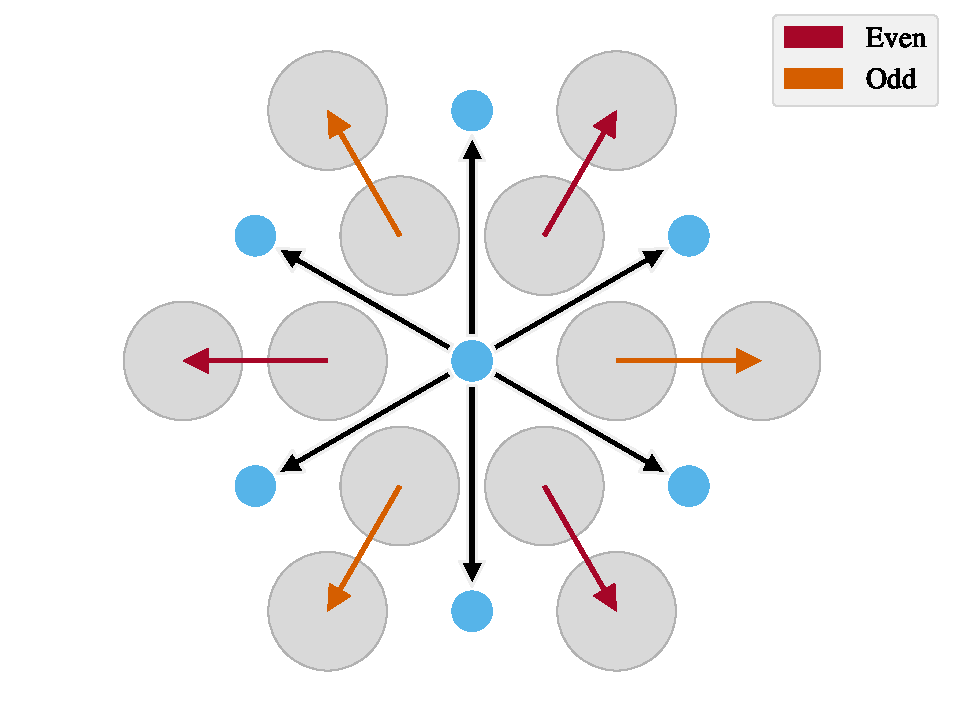
\includegraphics[width=0.5\linewidth]{figures/system/stay_or_break.pdf}
  \caption{...}
  \label{fig:stay_or_break}
\end{figure}


In cases where the site corresponding to following the previous direction is not available we get a break of direction by definition. 

\subsubsection{Deployment schemes} % Grid start, Centering, RN6
By default, each random walker is given an uniform random starting point among
the non-visited sites left on the sheet. This includes any modifications in
relation to the minimum distance parameter. By toggling the \textit{Grid start:
True/False} parameter on the starting points are instead predefined on evenly
spaced grid. That is, the sheet is subdivided into the least amount of squares
that will accomodate a space for each starting point. $\{1\}$ walker leads to a
$1\times 1$ partition, $\{2,3,4\}$ walkers lead to a $2\times 2$ partition,
$\{5,6,7,8,9\}$ walker lead to a $3\times 3$ partition and so on. The lower left
corner \footnote{In hindsight this would have been statistically better spaced
if with a random starting corner, but this is not considered to be of great
importance for the way we used this feature in the dataset generation.} is then choosen as a default starting place for the first
walker for which the remaining sites are filled according to the order that
maximizes the minimum distance between a new starting point and the ones already
used. The population of the grid is visualized in \cref{fig:grid_start} for 1-9 walkers in total. 


\begin{figure}[H]
  \centering
  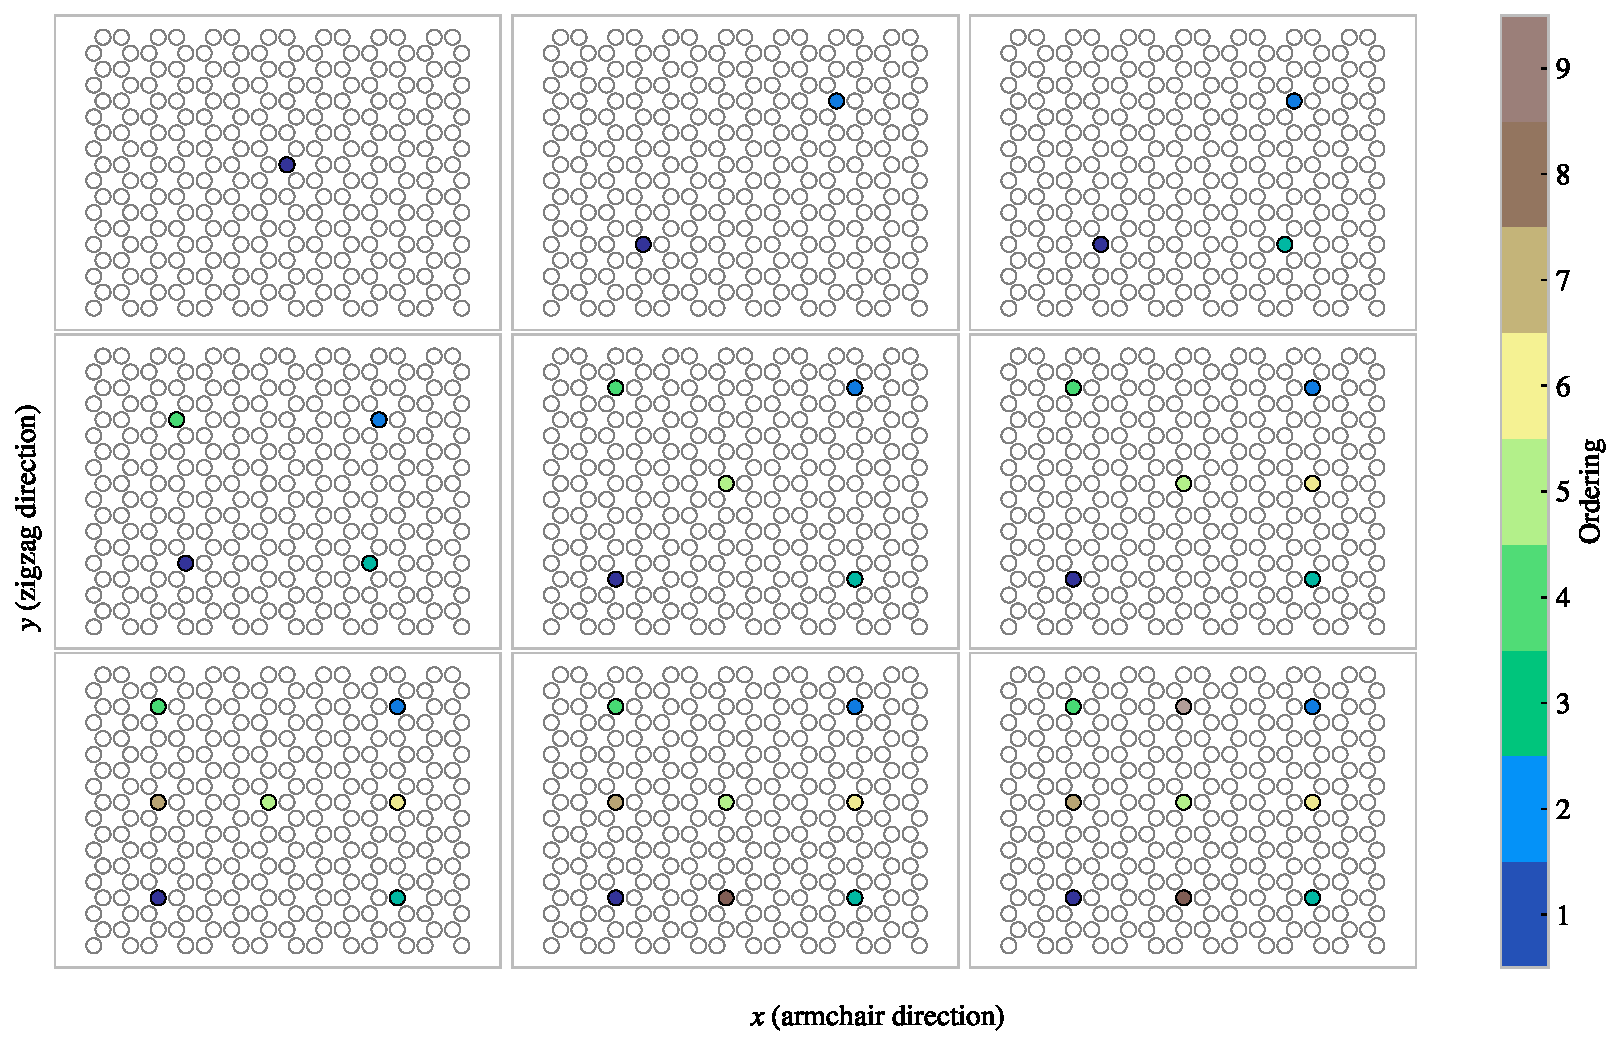
\includegraphics[width=\linewidth]{figures/system/grid_start.pdf}
  \caption{Populaiton of starting points with the centering parameter toggled on in a $14\times 18$ sheet. This is shown for 1-9 number of random walkers with the color map conveying the order of the population.}
  \label{fig:grid_start}
\end{figure}


The \textit{Centering: True/False} parameter let us relocate the path of the random walker such that the path center of mass alligns better with the starting point. This can be used in combination to the grid start and the bias parameter to make rather ordered configurations. In addition, the \textit{RN6:True/False} parameter can be used change the bias direction to on of the six directions of the center element walk for each new walker. This lets us create confgiratiosn like [EXAMPLE]. 

\subsubsection{Validity}
The simulation procedure requires the sheet is fully attatched which can be summarized as the following requirements. 
\begin{enumerate}
  \item There exist only a single cluster on the sheet. We define a cluster as the set of atoms which can all be reached through nearest neighbour walking on the cluster.
  \item The cluster of atoms is spanning the sheet in the y-direction. This means that there exist at least one path through nearest neighbour walks that connect the bottom and the top of the sheet. This is due to the reason that the sheet must be attatched to the pull blocks.
\end{enumerate}

In order to accommodate these requirements we count the number of clusters and search for a spanning cluster after all walkers have terminated. If the requirements are not met we simply rerun the random walk from scratch. This is done \textit{Avoid clustering} amount of times. If the requirements are not met during any of those reruns the non-spanning clusters are simply removed. In the case of no spanning cluster the configuration is dropped. This crude scheme was later reinvented as a more refined repair scheme which alters the sheet by the intention of performing the least amount of changes (addition of subtraction of atoms) in order to meet attatchment requirements. This was done as a part of the accelerated search procedure and hence it was not utilized in the creation of the random walk dataset. 



% We might get configurations with multiple isolated clusters, meaning that the sheet is already detached and the simulation will reach a halt immediately. This is especially a problem when having a high number of walkers with a high number of maximum steps. Even with the minimum distance parameter in use a single walker can sourround and inclose a region which will become detached. In order to mitigate this problem we count the number of clusters on the sheet after performing the random walks. We define a cluster of atoms as a set for which all atoms can be reached by walking between neighbouring sites. If there exist more than one cluster, or if the custer is not spanning the sheet in the x, y 



\subsubsection{Random walk examples}

\begin{figure}[H]
  \centering
  \includegraphics[width=\linewidth]{figures/system/RW_flavors.pdf}
  \caption{Some example uses of the random walking class.}
  \label{fig:RW_flavors}
\end{figure}
